%
%
%
\chapter{The static conductivity in the spin fermion model pertubated by umklapp scattering}
\label{ch: calculation}
%
%
%
In the last chapter the memory-matrix-formalism was introduced, which give us an exact formula to calculate correlation functions.
Now this formalism is used to determine the static conductivity of the spin-fermion-model, see chapter \ref{ch: spin fermion model}, pertubated by umklapp-scattering.
Firstly the static conductivity of the unpertubated spin-fermion-model is computed to remind and convience us that the conductivity is infinite in the case of unbroken translation symmetry.
Afterwards the translational symmetry is broken under consideration of umklapp scattering and the conductivity is calculated for this special case.
%
%
\section{Infinite conductivity in systems with unbroken translation symmetry}
\label{sec: Infinite conductivity in a system with unbroken translation symmetry}
%
%
After Drude published his theory about the electrical transport in metals \cite{Drude} in the beginning of the last century it is well known that a broken translation symmetry is needed to get a finite static conductivity.
Because of Neother's theorem \cite{Noether1} it is also well known that a unbroken symmetry always implies a conserved quantity.
In the case of translation symmetry this quantity is the momentum.
Phenomenas breaking the translation symmetry are for example impurity scattering, electron-electron scattering and umklapp scattering.
Let us firstly investigate the standard spin-fermion-model without a translation symmetry breaking pertubation.
In chapter \ref{ch: spin fermion model} it is showed that the unpertubated Hamiltonian conserves the momentum but dosen't conserves the current.
This property is utilized in the following calculation of the static conductivity.

In general the static conductivity is given by taking the small frequency limit of the conductivity and the conductivity itself is given by the current-current correlation function (J-J correlation function). This can be proven by assuming a oscillating electrical field and compute the expactaion value of the current via linear response theory, which is done in \cite{Chycholl2}.
%
\begin{align}
	\sigma_{\mt{dc}} = \lim\limits_{\omega \to 0} \sigma(\omega) = \lim\limits_{\omega \to 0}\, \beta\,\mathcal{C}_{\mt{JJ}}(\omega)
	\label{eq: general static condictivity}
\end{align}
%
Above in chapter \ref{ch: memory matrix formalism} the memory matrix formalism is derivated. 
Our main goal is to establish equation \eqref{eq: algebraic equation for C} which is an algebraic matrix equation for the correlation function.
Before the computation of $\mathcal{C}_{\mt{JJ}}(\omega)$ can be started we have to clarify the set of operators over which we sumarized.
The sums over $k$ and $l$ arise from the projection operator which means we have to discuss the Liouville subspace into the projection operator projects.
In general to choice of these operators has to be done for each calculation seperatly depending on the working model and the quantity of interest.
In the investigated case the electrical conductivity and the induction of umklapp scattering at the conductivity is computated.
As it is said above the electrical conductivity is proportional to the current operator, why this should be the first operator of our sought set of operators.
If an electrical field is applied the electrons accelareate because of the potential difference which increase the momentum of the electrons.
Thus the momentum is an inevitable quantity speaking about current and electrical conductivity this should be the second operator.
Beside these two operators now more operators are necessary.

The current and momentum have the same signature with respect to time reversal symmetry which simplifies the computation a lot.
Considering a invariant Hamiltonian under time reversal symmetrie.
Than in equation \eqref{eq: algebraic equation for C} $\Omega_{il}$ vanishes if both operators have the same signature under time reversal symmetry.
This assertion is proven in section \ref{subsec: time reversal symmetry} in detail.
In addition let do the investigation of $\Sigma_{il}$.
The expactation value is generated with respect to the derivative of an operator at each side.
On the right hand side the sum over $k$ has to be carried out which produces $\toket{\dot{\mt{P}}}$ and $\toket{\dot{\mt{J}}}$.
The first one is trivially zero, because the momentum is a conserved quantity.
The latter has to be investigated under the action of the operator $\mt{Q}$, which projected out off the J-P-subspace.
$\mt{Q}\toket{\dot{\mt{J}}}$ describes the coupling on all the other degrees of freedom in the system, which is zero in the considered system.
With all these simplifications equation \eqref{eq: algebraic equation for C} yields
%
\begin{align}
	\begin{pmatrix}
	\mathcal{C}_{\mt{JJ}}(\omega) &  \mathcal{C}_{\mt{JP}}(\omega) \\
	\mathcal{C}_{\mt{PJ}}(\omega) &  \mathcal{C}_{\mt{PP}}(\omega)
	\end{pmatrix}
	=
	\frac{i}{\beta}
	\begin{pmatrix}
	\omega^{-1} & 0 \\
	0 & \omega^{-1} 
	\end{pmatrix}
	\cdot
	\begin{pmatrix}
	\chi_{\mt{JJ}}(\omega) &  \chi_{\mt{JP}}(\omega) \\
	\chi_{\mt{PJ}}(\omega) &  \chi_{\mt{PP}}(\omega)
	\end{pmatrix}.
\end{align}
%
The current current correlation function is given by
%
\begin{align}
	\mathcal{C}_{\mt{JJ}}(z) = \frac{i}{\beta} \omega^{-1} \chi_{\mt{JJ}}(\omega=0) = \frac{i}{\omega} \mathcal{C}_{\mt{JJ}}(t=0),
	\label{eq: correlation function unpertubated system}
\end{align}
%
where relation \eqref{eq: relation between C, Phi and chi} is used.
The correlation function at $t = 0$ is given by the scalar product $\tobraket{\mt{J}(0)}{\mt{J}(0)}$, see equation \eqref{eq: correlation function Liouville space}.
Nothing or nobody bars us from splitting the vector operator $\toket{\mt{J}(0)}$ into two pieces, one parallel and one vertical part, which corresponds to the secular and non-secular part of the observable, respectivily.
Formaly this look like
%
\begin{align}
	\oket{\mt{J}} = \oket{\mt{J}_{\mid\mid}} + \oket{\mt{J}_{\bot}}.
	\label{eq: splitting current}
\end{align}
%
In general every observable can be consist a conserved and a non-conserved part, what shouldn't mean that both parts exist in every investigated system.
Dissipative prozesses like fluctuations or initial transient processes for example are included in the non-conserved part.
These non-secular effects are visible as noise in the experiement and the vertical part of the vector is indetified with these kinds of prozesses.
Apart from this the secular conserved part of the observable is represented by the parallel part of $\toket{\mt{J}}$.
In Drude's theory of conductivity the current is proportional to the momentum in the way that $j = -\frac{en}{m}p$.
In the spin fermion model, see chapter \ref{ch: spin fermion model}, the momentum is conserved but the current isn't conserved, which means that the conductivity can't given by Drude's theory at all.
Nevertheless because the momentum is conserved the conserved part of the current has to be in the direction of the momentum.
In mathematical language this means that the parallel part of the current $\toket{\mt{J}_{\mid\mid}}$ is the projection from $\toket{\mt{J}}$ onto $\toket{\mt{P}}$.
%
\begin{align}
	\oket{\mt{J}_{\mid\mid}} = \mathcal{P}\oket{\mt{J}} = \frac{\odyad{\mt{P}}{\mt{P}}}{\obraket{\mt{P}}{\mt{P}}} \oket{\mt{J}} = \frac{\chi_{\mt{PJ}}}{\chi_{\mt{PP}}} \oket{\mt{P}}
	\label{eq: parallel current as projection}
\end{align}
%
This give us the oppertunity to write the J-J correlation function into two parts one parrallel and one perpendicular correlation function where equation \eqref{eq: splitting current} is used.
The mixed correlation functions are zero by construction, because $\toket{\mt{J}_{\mid\mid}}$ and $\toket{\mt{J}_{\bot}}$ are orthogonal and therfore the terms vanish.
%
\begin{align}
	\mathcal{C}_{\mt{JJ}}(t=0) = \obraket{\mt{J}(0)}{\mt{J}(0)} = \obraket{\mt{J}_{\mid\mid}}{\mt{J}_{\mid\mid}} + \obraket{\mt{J}_{\bot}}{\mt{J}_{\bot}}
\end{align}
%
Equation \eqref{eq: parallel current as projection} is used to express the parallel J-J correlation function as a momentum-momentum correlation function (P-P correlation) formaly given by $\tobraket{\mt{P}}{\mt{P}}$.
%
\begin{align}
	\mathcal{C}_{\mt{JJ}}(t=0) = \frac{\vert\chi_{\mt{PJ}}\vert^{2}}{\vert\chi_{\mt{PP}}\vert^{2}} \mathcal{C}_{\mt{PP}}(t=0) + \obraket{\mt{J}_{\bot}}{\mt{J}_{\bot}}
\end{align}
%
Using \eqref{eq: relation between C, Phi and chi} and insert back this expression in equation \eqref{eq: correlation function unpertubated system} which give us multipled with $\beta$ the conductivity
%
\begin{align}
	\sigma (z) = \frac{\vert\chi_{\mt{PJ}}\vert^{2}}{\vert\chi_{\mt{PP}}\vert} \frac{i}{\omega}  + \sigma_{\mt{reg}}(\omega)
\end{align}
%
%
\begin{figure}[t]
	\subfigure[conductivity in a system with unbroken translation symmetry]{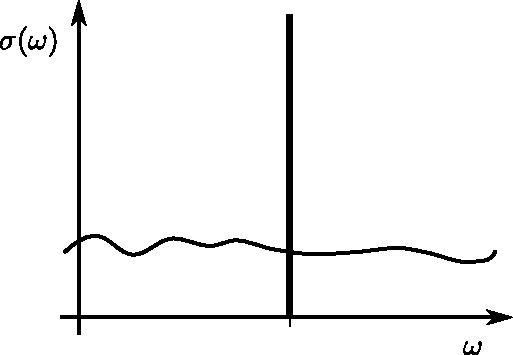
\includegraphics[width=0.45\textwidth]{conductivity_delta_peak.pdf}}
	\subfigure[conductivity in a system with broken translation symmetry]{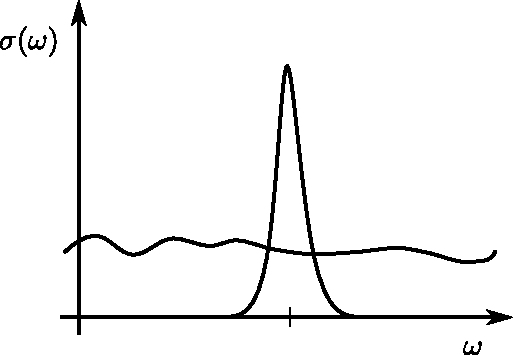
\includegraphics[width=0.45\textwidth]{conductivity_drude_peak.pdf}}
	\caption{caption}
	\label{fig: conductivity broken and unbroken translation symmetry}
\end{figure}
%
where the regular conductivity $\sigma_{\mt{reg}}(z) = \frac{i \beta}{\omega} \obraket{\mt{J}_{\bot}}{\mt{J}_{\bot}}$ is introduced.
The physical meaning of $\sigma_{\mt{reg}}(\omega)$ is directly connected to the vertical component of $\toket{\mt{J}}$.
Thus the regular conductivity includes fluctuations and other effects influenced by random forces called noise.
Figure \ref{fig: conductivity broken and unbroken translation symmetry} shows this continuously over all frequencies never disappearing background.

In the whole calculation never a condiction on $\omega$ is made, so the equation for the conductivity is valid for each $\omega$ in the complex plane.
In reality the conductivity isn't depending on a complex frequency, because physical quantities are always real.
Therefore we have to set $\omega = \omega + i \eta$, where now $\omega \in \mathbb{R}$ and the limit $\eta \to 0$ is implied.
Using $\frac{1}{\omega + i\eta} = \PV{\frac{1}{\omega}} - i\pi\delta(\omega)$ the conductivity is given by
%
\begin{align}
	\sigma(\omega) = \frac{\vert\chi_{\mt{PJ}}\vert^{2}}{\vert\chi_{\mt{PP}}\vert} \bigg(\PV{\frac{i}{\omega}} + \pi \delta(\omega) \bigg) + \sigma_{\mt{reg}}(\omega)
	\label{eq: conductivity unpertubed system}
\end{align}
%
where $\PV$ sympolizied that the prinzipal value is taken.
Equation \eqref{eq: conductivity unpertubed system} yields exactly the expected result.
For small frequencies the main contribution is generated by the $\delta$-distribution, so the conductivity becomes infinite.
This is the expected result, because the translation symmetry isn't broken in the investigated system.
If voltage is applied on a system with unbroken translational symmetry the electrons accelerate infinite long.
There is nothing they can scatter on and therefore nothing to lose momentum.
The electrons accelerate more and more and this eventuates in an infinite conductivity.
Only in a system with broken translation symmetry it's possible for the electrons to lose momentum by scattering with the lattice or impurities for example.
This eventuates in a finite conductivity, thus the amplitude of the $\delta$-peak becomes smaller or more precisely finite.
The factor in front of the $\delta$-distribution is the so called Drude weight.
The Drude peak and the effect of breaking translation symmetry is visualizied in figure \ref{fig: conductivity broken and unbroken translation symmetry} too.
%
%
\section{Finite conductivity because of breaking the translation symmetry via umklapp scattering}
\label{sec: finite conductivity because of breaking the translation symmetry via umklapp scattering}
%
%
The conservation of momentum connected with an unbroken translation symmetry yields a infinite electrical conductivity, which is computated in the previous section.
In the next calculation a system with broken translation symmetry is considered.
The assumed symmetry breaking pertubation is umklapp scattering, where the Hamiltonian is given by equation (\todo{link zu umklapp hamiltonian}).
In \dots\todo{link zum abschnitt in dem gezeigt wird das P nicht mehr erhalten ist} it is shown that this pertubation is the reason for an unconserved momentum.
Thus the above disscusion about the Drude weight and conductivity let us expect that the conductivity is lessened to a finite value.
The static electrical conductivity is given by equation \eqref{eq: general static condictivity} in general.
Again the memory matrix formalsim is now used to compute the current-current correlation function given by the formal equation
%
\begin{align}
	\sum\limits_{l} \Big[\omega \delta_{il} - \Omega_{il} + i \Sigma_{il}(\omega)\Big] \mathcal{C}_{lj}(\omega) = \frac{i}{\beta} \chi_{ij}(0)
\end{align}
%
where $\Omega_{il}$ and $\Sigma_{il}(\omega)$ are given by
%
\begin{align}
	&\Omega_{il} = i \beta \sum\limits_{k} \obraket{\dot{\mt{A}}_{i}}{\mt{C}_{k}} \chi_{kl}^{-1}(0) \qq{and} \\
	&\Sigma_{il}(\omega) = i \beta \sum\limits_{k} \obra{\dot{\mt{A}}_{i}} \mt{Q} \frac{1}{\omega - \mt{QLQ}} \mt{Q} \oket{\dot{\mt{C}}_{k}} \chi_{kl}^{-1}(0).
\end{align}
%
Always the first step is to think about the vector subspace, generated by the vectors of the projection operator.
Computing the electrical conductivity the current and the momentum operator are usually the operators of interest. \todo{vllt noch etwas ausf\"uhrlicher schreiben}
Therefore our decision is made and our subspace is generated by these two operators.
What does this choice of operators mean for the quantities $\Omega_{il}$ and $\Sigma_{il}(\omega)$?
Starting with the first one.
$\Omega_{il}$ vanishs if two properties are valid.
The first one is, that the considered Hamiltonian has to be invariant with respect to time reversal symmetry.
The unpertubated Hamiltonian (\dots\todo{link zum ungest\"orten Hamiltonian}) and the pertubation Hamiltonian (\dots\todo{link zum umklapp Hamiltonian}) occupy this condiction which is trivially to prove.
The second property is that both operators labeled with $\mt{A}_{i}$ and $\mt{C}_{k}$ must have the same signature under time reversal symmetry.
Both operators can be either $\mt{J}$ or $\mt{P}$, where both have the same signature under time reversal symmetry.
Therefore in all cases the quantity $\Omega_{il}$ is zero.
In $\Sigma_{il}(\omega)$ the expecation value is formed with respect of the derivative of vector operators, which are $\toket{\dot{\mt{J}}}$ and $\toket{\dot{\mt{P}}}$.
In the discussion above a translation invariant system is assumed why the derivative of the momentum vanishes.
Now the momentum isn't anymore conserved and therefore the derivative yields a finite value.

For further assertions the action of the operator $\mt{Q}$ has to be investigated on both vector operator.
$\mt{Q} \toket{\dot{\mt{C}}_{k}}$ describes the coupling to all other degrees of freedom which aren't included in the subspace.
Firstly remember that umklapp scattering is the considered pertubation.
What does this pertubation change in our system?
It breaks translation symmetry which yields some finite value for $\dot{\mt{P}}$ instead of zero in the unpertubated system.
This means the complete unconserved part of the momentum is coupled to the crystal lattice which is clearly a degree of freedom out off the J-P subspace.
This is the reason why $\mt{Q} \toket{\dot{\mt{P}}} = \toket{\dot{\mt{P}}}$.
Further the pertubation doesn't change the quantity $\toket{\dot{\mt{J}}}$.
The unconserved current yields from the interaction between the electrons lives on different Fermi surfaces coupeld via spin density waves.
This process is included in the J-P subspace and therefore $\mt{Q} \toket{\dot{\mt{J}}} = 0$.
This signifies for the memory function that $\Sigma_{il}$ doesn't vanish if $i=\mt{P}$ and vanish if $i=\mt{J}$.

In summary umklapp scattering yields a non-zero contribution to the memory function $\Sigma_{il}(\omega)$ and is therefore a correction of the correlation function instead of the unpertubated case where the memory function is zero.
Equation \eqref{eq: algebraic equation for C} yields 4 equations in the J-P subspace, which can be writen as a matrix equation.
%
\begin{align}
	\begin{pmatrix}
	\omega & 0 \\
	-i\Sigma_{\mt{PJ}}(\omega) & \omega - i\Sigma_{\mt{PP}}(\omega)
	\end{pmatrix}
	\cdot
	\begin{pmatrix}
	\mathcal{C}_{\mt{JJ}}(\omega) &  \mathcal{C}_{\mt{JP}}(\omega) \\
	\mathcal{C}_{\mt{PJ}}(\omega) &  \mathcal{C}_{\mt{PP}}(\omega)
	\end{pmatrix}
	=
	\frac{i}{\beta}
	\begin{pmatrix}
	\chi_{\mt{JJ}}(0) &  \chi_{\mt{JP}}(0) \\
	\chi_{\mt{PJ}}(0) &  \chi_{\mt{PP}}(0)
	\end{pmatrix}
	\label{eq: matric equation correlation function unconserved momentum}
\end{align}
%
Before the computation is going on we want to make a short remark.
Equation \eqref{eq: algebraic equation for C} is an exact algebraic matrix equation.
At the derivation no assumtions are made and up to this point we have also made no assumptions.
All the conversion we have done are exact and only depending on the considered model.

The electrical conductivity is given by the J-J correlation function, which has the formal expression
%
\begin{align}
	\mathcal{C}_{\mt{JJ}}(\omega) = \obra{\mt{J}} \frac{i}{\omega - \mt{L}} \oket{\mt{J}}
\end{align}
%
in frequenzy space.
Equally to the case of conserved momentum nothing bars us to split the current into one parallel and one vertical part, where the parallel part is pointed in the direction of the secular component of J.
The appearing mixed correlation functions vanishes because $\toket{\mt{J}_{\mid\mid}}$ and $\toket{\mt{J}_{\bot}}$ are orthogonal.
How we have seen in the previous section the background or noise originated by fluctuation and other random processes, which is represented by the correlation function of the vertical component.
This term isn't necessary to write it down every time why we drop it.
%A theoretical phyisicist would say that the origin is always taken arbitrary.
%A experimental phyisicist would say that he calibrates the measurement.
For a discussion in more detail the work of Jung \cite{Jung} is suggested.
However the only important part for us is the parallel component of the correlation function.
On the other hand the parallel componend of the correlation function is given by the projection of J onto P, see equation \eqref{eq: parallel current as projection}.
Thus the J-J correlation function is rewriten in a P-P correlation function mutiplied with a fraction of susceptibilities.
%
\begin{align}
	\mathcal{C}_{\mt{JJ}}(\omega) = \obra{\mt{J}_{\mid\mid}} \frac{i}{\omega - \mt{L}} \oket{\mt{J}_{\mid\mid}} = \frac{\vert\chi_{\mt{PJ}}\vert^{2}}{\vert\chi_{\mt{PP}}\vert^{2}} \mathcal{C}_{\mt{PP}}(\omega)
\end{align}
%
The P-P correlation function can be readed out of equation \eqref{eq: matric equation correlation function unconserved momentum}.
Therefore the inverse of the memory matrix has to be multiplied from the left hand side.
The P-P correlation function is then given by
%
\begin{align}
	\mathcal{C}_{\mt{PP}}(\omega) = \frac{i}{\beta} \cdot \frac{i \Sigma_{\mt{PJ}}(\omega)  \chi_{\mt{JP}}(0)}{\omega\big(\omega - i\Sigma_{\mt{PP}}(\omega)\big)} + \frac{i}{\beta} \cdot \frac{\chi_{\mt{PP}}(0)}{\omega - i\Sigma_{\mt{PP}}(\omega)} \approx \frac{i}{\beta} \cdot \frac{i \chi_{\mt{PP}}(0)}{\Sigma_{\mt{PP}}(\omega)}
\end{align}
%
where in the last step the limit of small frequencies is taken.
Then on the one hand the first term is neglectable compared to the second one. \todo{Why?}
On the other hand is $\omega \ll \Sigma_{\mt{PP}}(\omega)$.
Thus in the second term $\omega$ is neglectable against $\Sigma_{\mt{PP}}(\omega)$.
In summary the static conductivity is given by
%
\begin{align}
	\sigma_{\mt{dc}} = \lim\limits_{\omega \to 0} \beta \mathcal{C}_{\mt{JJ}}(\omega) = \frac{i}{\beta} \lim\limits_{\omega \to 0} \frac{\vert\chi_{\mt{PJ}}\vert^{2}}{\chi_{\mt{PP}}} \frac{i \beta}{\Sigma_{\mt{PP}}(\omega)}
\end{align}
%
The memory function $\Sigma_{\mt{PP}}(\omega)$ is definied in equation \eqref{eq: Sigma(z)}.
Because of the considered Hamiltonian only the term included $\dot{\mt{P}}$ yields a non-zero contribution.
Further the operator $\mt{QLQ}$ can be approximated by $\mt{L}_{0}$ the Liouville operator of the unpertubated system. \todo{Warum darf QLQ mit $L_{0}$ approximiert werden?}
The final expression for the dc-conductivity is given by
%
\begin{align}
	\sigma_{\mt{dc}} \approx \frac{i}{\beta} \lim\limits_{\omega \to 0} \vert\chi_{\mt{PJ}}\vert^{2} \obra{\dot{\mt{P}}} \frac{1}{\omega - \mt{L_{0}}} \oket{\dot{\mt{P}}}^{-1}
\end{align}
%
In a short conversion the expectation value can be expressed as a time integral over the $\dot{\mt{P}}$-$\dot{\mt{P}}$ susceptibility.
This expression is more usefull for explicite computations, because it allows us using pertubation theory.
For the detailed conversion see appendix \ref{app: conversion expval}.
The static electrical conductivity is finaly given by
\todo{$-\hbar$???}
%
\begin{align}
	\sigma_{\mt{dc}} \approx -\hbar \lim\limits_{\omega \to 0} \frac{\omega \vert \chi_{\mt{JP}}(\omega = 0) \vert^{2}}{\int\limits_{0}^{\infty} \dd{t} e^{i\omega t} \expval{\comm{\dot{\mt{P}}(t)}{\dot{\mt{P}}(0)}}_{0}},
	\label{eq: formula static conductivity}
\end{align}
%
which is used in the compuation below.
The calculation is splitted into two parts.
At first the computation of the denominator is perfermed, which gives us the temperature dependence of the conductivity.
Further the J-P susceptibility has to be calculated.
In first order for this quantity is expected no temperature dependence, but we have to convience us from this.
%
%
\subsection{Temperature dependence of the dc-conductivity}
\label{subsec: temperature dependence of the dc-conductivity}
%
%
Our starting point is the integral in the denominator of the last equation above.
The index $0$ at the expectation value means that it has to be computed with respect to the equilibrium Hamiltonian $\mt{H}_{1} = \mt{H}_{\Psi} + \mt{H}_{\Phi} + \mt{H}_{\Psi\Phi}$.
The considered umklapp scattering is only entered in the time derivative of the momentum.
Commonly the sort of this calculation is done in the Matsubara time $\tau = it$, see e.\,g. \cite{Bruus&Flensberg} for an introduction or a review.
%
\begin{align}
	\mathcal{G}_{jj}(z) :=  \int\limits_{0}^{\infty} \dd{t} e^{iz t} \expval{\comm{\dot{\mt{P}}_{j}(t)}{\dot{\mt{P}}_{j}(0)}}_{\mt{H}_{1}} = i \int\limits_{0}^{\beta} \dd{\tau} e^{z \tau} \expval{\mathcal{T}_{\tau} \dot{\mt{P}}_{j}(\tau) \dot{\mt{P}}_{j}(0)}_{\mt{H}_{1}}
\end{align}
%
The norm of the Jacobi determinate is $-i$ and the upper integral limit changes from infinity to $\beta$.
Further each time derivative yields an $i$.
Totally the factor $i$ is multiplied to the integral.
The direction of the momentum is denoted with the index $j$ and to symbolisied clearly that the frequency is an arbitrary number in the complex plane the variable $z$ is used instead of $\omega$.
Like it is done every time in pertubation theory the operators are transformed into the Matsubara interaction representation.
The transformation's aim is that the expectation value is only taken with respect to the free Hamiltonian $\mt{H}_{0} = \mt{H}_{\Psi} + \mt{H}_{\Phi}$ and the interation $\mt{H}_{\Psi\Phi}$ is only entered in the time evolution operator $\mt{U}(\beta,0)$.
A series expansion of this one up to the first non-disappearing order yields
%
\begin{align}
	\mathcal{G}_{jj}(z) = i \int\limits_{0}^{\beta} \dd{\tau} e^{z \tau} \expval{\mathcal{T}_{\tau} \dot{\mt{P}}_{j}(\tau) \dot{\mt{P}}_{j}(0)}_{\mt{H}_{0}}^{\mt{con}}
\end{align}
%
where it has to be remarked that in quantum field pertubation theory only connected diagrams are considered, which is indicated with "con" at the expectation value.
At the numerator all disconnected diagrams can be factorizied.
These diagrams are exactly the same one as in the denominator, so both cancel each other.

In chapter \ref{ch: spin fermion model} umklapp scattering is introduced as a pertubation of the spin fermion system described by $\mt{H}_{1}$.
On the basis of this pertubation the momentum isn't anymore conserved, thus the time derivative of the momentum doesn't vanish.
The time derivative of an operator is given via the Heisenberg equation of motion, which yields in case of momentum
%
\begin{align}
	\dot{\mt{P}}_{j}(\tau) = \frac{i}{\hbar} \sum\limits_{\vb{K}} \mt{J}_{\vb{K}} \int_{\vb{k}} K_{j} \Phi_{\mu}(\vb{k},\tau) \Phi_{\mu}(-\vb{k} - \vb{K},\tau)
\end{align}
%
where $j$ indicated the direction of the momentum.
The sum over $\mu$ is implied.
Inserting the time derivative of the momentum in $\mt{I}_{jj}(z)$ yields
%
\begin{align}
	\mathcal{G}_{jj}(z) &= 
		-\frac{i}{\hbar^{2}} 
		\sum\limits_{\vb{K}_{1}, \vb{K}_{2}} 
		\mt{J}_{\vb{K}_{1}} \mt{J}_{\vb{K}_{2}} 
		\int\limits_{0}^{\beta} \dd{\tau} e^{z \tau} 
		\int_{\vb{k}_{1}}\int_{\vb{k}_{2}} K_{1,j}  K_{2,j} 
		\notag \\
		&\times
		\expval{\mathcal{T}_{\tau} \Phi_{\mu}(\vb{k}_{1},\tau) \Phi_{\mu}(-\vb{k}_{1} - \vb{K}_{1},\tau) \Phi_{\lambda}(\vb{k}_{2},0) \Phi_{\lambda}(-\vb{k}_{2} - \vb{K}_{2},0)}_{\mt{H}_{0}}
\end{align}
%
The expactation value is evaluated by using Wick's theorem, where the expactation value is related to the ground state of the system.
Therefore all normal products are zero and only the sum survives, where all operators are contracted.
The sum yields three possible contraction of the operators, where one of them is a disconnected diagram.
The diagram is originated by contracting the operators with the same time argument.
This diagram is canceled with the vacuum diagrams like discussed above, because it isn't considered in the following computation.
In total Wick's theorem yields two contributing diagrams, where both are equally.
The diagram is depicted in figure \ref{fig: spin wave bubble} and corresponds to the bubble diagram.

Because the used operators are in momentum space each expactation value of two operators becomes a $\delta$-distribution, originated from the commutator relations in momentum space.
The $\delta$-distributions signify the conservation of momentum.
In the investigated case the commutator relations \dots \todo{Link zu kommutator relationen} have to be used.
Then one momentum integral and one sum over reziprocal lattice vectors is performed.
The remaining momentum and reziprocal lattice vector is renamed into $\vb{k}$ and $\vb{K}$ respectivily.
Further one sum over the spactial direction of $\Phi$ is performed.
%
\begin{figure}
	\centering
	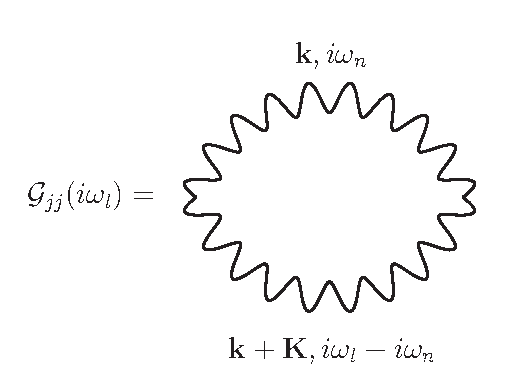
\includegraphics[width=0.5\textwidth]{spin_wave_bubble.eps}
	\caption{caption}
	\label{fig: spin wave bubble}
\end{figure}
%
%
\begin{align}
	\mathcal{G}_{jj}(z) &= 
		-\frac{2}{\hbar^{2}} 
		\sum\limits_{\vb{K}} 
		\vert \mt{J}_{\vb{K}} \vert^{2}
		\int\limits_{0}^{\beta} \dd{\tau} e^{z \tau} 
		\int_{\vb{k}} K_{j}^{2}
		\notag \\
		&\times
		\expval{\mathcal{T}_{\tau} \Phi_{\mu}(\vb{k},\tau) \Phi_{\mu}(-\vb{k},0)}_{\mt{H}_{0}} 
		\expval{\mathcal{T}_{\tau} \Phi_{\mu}(-\vb{k} - \vb{K},\tau) \Phi_{\mu}(\vb{k}+\vb{K},0)}_{\mt{H}_{0}},
\end{align}
%
where $\mt{J}_{-\vb{K}} = \mt{J}_{\vb{K}}^{*}$ is used. 
The asterisk denotes the complex conjugated.
Every single expectation value corresponds to the free propagator of spin density waves.
The free propagator is defined by $\mathcal{D}_{\mu}^{(0)}(\vb{k},\tau) := \expval*{\mathcal{T}_{\tau} \Phi_{\mu}(\vb{k},\tau) \Phi_{\mu}(-\vb{k},0)}_{\mt{H}_{0}}$.
Both are seperatly transformed into Matsubara frequency space via
%
\begin{align}
	\mathcal{D}_{\mu}^{(0)}(\vb{k},\tau) = \frac{1}{\beta} \sum\limits_{\omega_{n}} e^{-i\omega_{n}\tau} \mathcal{D}_{\mu}^{(0)}(\vb{k},i\omega_{n})
\end{align}
%
where the summation runs over all Matsubara frequencies $\omega_{n}$.
Because the transformation rotates our investigated function onto the imaginary frequency axis, the complex frequency $z$ has to be set to $i\omega_{l}$.
After transforming the propagators into Matsubara frequency space the imaginary time dependence is solely originated from the exponential functions.
This offers us to perform the $\tau$-integral easily, where relation 
%
\begin{align}
	\int_{0}^{\beta} \dd{\tau} e^{-i(\omega_{m}+\omega_{n}-\omega_{l})\tau} = \beta \delta_{\omega_{m}+\omega_{l}-\omega_{n}}
\end{align}
%
is used and then one of the two sums over Matsubara frequencies can be performed as well.
After all these steps the integral has the form
%
\begin{align}
	\mathcal{G}_{jj}(i\omega_{l}) &= 
		-\frac{2}{\hbar^{2}} 
		\sum\limits_{\vb{K}} 
		\vert \mt{J}_{\vb{K}} \vert^{2}
		\int_{\vb{k}} K_{j}^{2}
		\frac{1}{\beta} \sum\limits_{\omega_{n}}
		\mathcal{D}_{\mu}(\vb{k},i\omega_{n}) \,
		\mathcal{D}_{\mu}(-\vb{k}-\vb{K},i\omega_{l}-i\omega_{n})
		\label{eq: Green function on the imaginary axis}
\end{align}
%
In the following the Matsubara sum is evaluated.
Therefore we have to check the singularities of both propgators.
Regarding equation \eqref{eq: damped propagator Matsubara representation}, illustrates that the propagator has a discontinuity if the absoulte value of the Matsubara frequency is zero.
%
\begin{figure}[t]
	\centering
	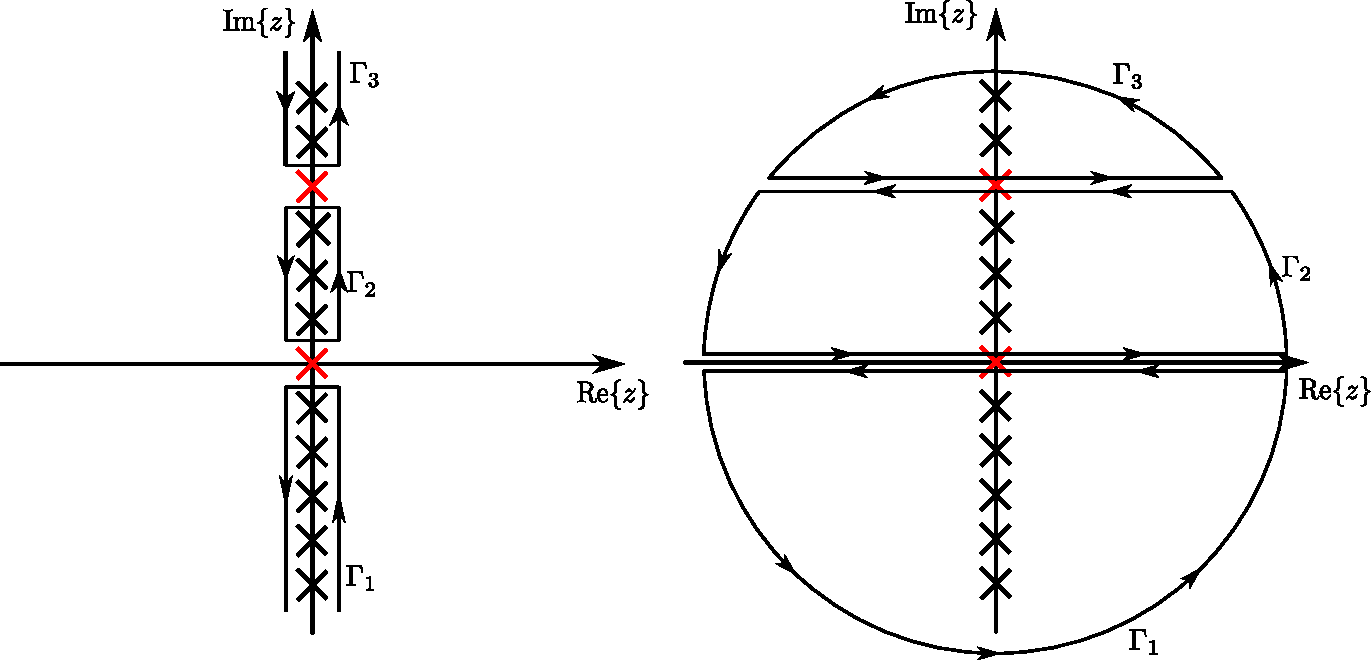
\includegraphics[width=\textwidth]{contour_branch_cut.pdf}
	\caption{caption}
	\label{fig: contour branch cut}
\end{figure}
%
This kind of singularity is called branch cut, because the whole horizontal line at the singularity is forbidden in the complex plane.
Branch cuts are the reason why the Matsubara sum isn't so easily transformed into a complex contour integral like it is done usually, if the propagators have simple poles.
In the investigated case the propagators have two singularity of this kind, one at $\omega_{n} = 0$ and one at $\omega_{n} = \omega_{l}$, which correspond to $n=0$ and $n=l$.
The strategy to evaluate those Matsubara sums is to seperate the singularities from the sum.
For reasons of simplizity the momentum argument of the second propagator is abbreviatied as $\vb{k}'=-\vb{k}-\vb{K}$ and the momentum argument is written in both cases as an index until the Matsubara sum is evaluated.
%
\begin{align}
	S(i\omega_{l}) :&= \frac{1}{\beta} \sum\limits_{\omega_{n}} \mathcal{D}_{\mu,\vb{k}}(i\omega_{n}) \, \mathcal{D}_{\mu,\vb{k}'}(i\omega_{l}-i\omega_{n})
	\notag \\
	\Leftrightarrow\ S(i\omega_{l}) :&= 
		\frac{1}{\beta} \mathcal{D}_{\mu,\vb{k}}(0) \, \mathcal{D}_{\mu,\vb{k}'}(i\omega_{l})
		+
		\frac{1}{\beta} \mathcal{D}_{\mu,\vb{k}}(i\omega_{l}) \, \mathcal{D}_{\mu,\vb{k}'}(0)
		\notag \\
		&+
		\frac{1}{\beta} \sum\limits_{\substack{n \neq 0 \\ n \neq l}} \mathcal{D}_{\mu,\vb{k}}(i\omega_{n}) \, \mathcal{D}_{\mu,\vb{k}'}(i\omega_{l}-i\omega_{n})
	\label{eq: seperated Matsubara sum}
\end{align}
%
Now the remaining sum can be transformed into a complex contour integral.
Thereby the contour $\Gamma$ includes all Matsubara frequencies $\omega_{n}$ onto the imaginary axis, beside the two ones splitted off, and is taken counterclockwise.
The contour $\Gamma$ is depicted in figure \ref{fig: contour branch cut}.
The transformed Matsubara sum is given by
%
\begin{align}
	\mt{I}_{MS}(\omega_{l}) := 
		\frac{1}{\beta} \sum\limits_{\substack{n \neq 0 \\ n \neq l}} \mathcal{D}_{\mu,\vb{k}}(i\omega_{n}) \, \mathcal{D}_{\mu,\vb{k}'}(i\omega_{l}-i\omega_{n})
		=
		\oint\limits_{\Gamma} \frac{\dd{z}}{2\pi i} n_{\mt{B}}(z) \mathcal{D}_{\mu,\vb{k}}(z) \, \mathcal{D}_{\mu,\vb{k}'}(i\omega_{l}-z),
\end{align}
%
where $n_{\mt{B}}(z)$ is the Bose distribution.
Like it is shown in \ref{fig: contour branch cut} $\Gamma$ consists of three single contours which are denoted as $\Gamma_{1}$, $\Gamma_{2}$ and $\Gamma_{3}$.
These three contours are expanded to infity where the contour line is never allow to cross the horizontal line at $\omega_{l}$ and $0$.

The contour $\Gamma_{1}$ is taken along the real axis in negative direction and is closed by a semi-circle with infinite radius in the lower complex plane.
$\Gamma_{2}$ is the contour between both branch cuts.
Starting the contour along the real axis in positive direction.
At infinity the contour is going up to the branch cut at $\omega_{n}$, along this axis back to minus infinity and finally back down to the starting point.
The last contour $\Gamma_{3}$ is going along the $\omega_{n}$-axis in positive direction and is closed by a semi-circle with infinite radius in the upper complex plane.
The contour along the real and $\omega_{n}$-axis has to be set infinitesimal beside the axis, which is indicated with the term $\pm i\eta$.
The sign has to be chosen according to the contour.

Each one of these three contour integrals can be splitted in parts.
The contours $\Gamma_{1}$ and $\Gamma_{3}$ is seperated into the path along the real or $\omega_{l}$-axis, respectivily, and the corresponding semi-circle.
In both cases the contribution of the semi-circles vanish, because the integrand decreases faster than $\flatfrac{1}{z}$.
In total $\Gamma_{2}$ is seperated into four parts.
Two parts are the paths along the real and $\omega_{l}$-axis.
The other both paths are the connecting path between them.
Equally to the case of the semi-circles these two path vanish.
In summary only the paths along the two branch cuts survive.
%
\begin{align}
	\mt{I}_{MS}(\omega_{l}) &= 
		\int\limits_{-\infty}^{\infty} \frac{\dd{\epsilon}}{2\pi i} 
			\mathcal{D}_{\mu,\vb{k}'}(i\omega_{l}-\epsilon)
			\bigg[
				n_{\mt{B}}(\epsilon - i\eta) 
				\mathcal{D}_{\mu,\vb{k}}(\epsilon - i\eta) 
				- 
				n_{\mt{B}}(\epsilon + i\eta) 
				\mathcal{D}_{\mu,\vb{k}}(\epsilon + i\eta)
			\bigg]
		\notag \\ &+
		\int\limits_{-\infty}^{\infty} \frac{\dd{\epsilon}}{2\pi i} 
			\mathcal{D}_{\mu,\vb{k}}(i\omega_{l} + \epsilon)
			\bigg[
				n_{\mt{B}}(i\omega_{l} + \epsilon - i\eta)  
				\mathcal{D}_{\mu,\vb{k}'}(\epsilon - i\eta) 
				\notag \\& \hspace{3.6cm}- 
				n_{\mt{B}}(i\omega_{l} + \epsilon + i\eta)
				\mathcal{D}_{\mu,\vb{k}'}(\epsilon + i\eta)
			\bigg]
	\label{eq: Matsubara sum along axes parallel to real axis}
\end{align}
%
where the limit $\eta \to 0^{+}$ is implied.
Further we used that the propagator $\mathcal{D}$ is symmetric with respect to the frequency argument.
It is easy to prove that $n_{\mt{B}}(z+i\omega_{l}) = n_{\mt{B}}(z)$, which means that the Bose distribution is invariant with respect to Matsubara frequencies.
Thereby is $z \in \mathbb{C}$ and $\omega_{l} = \flatfrac{2\pi l}{\beta}$ with $l \in \mathbb{Z}$ is a bosonic Matsubara frequency and therefore $\exp(i\omega_{l}) = 1$.
Now we set $z = \epsilon \pm i\eta$ and investigate the Bose distribution with respect to the limit $\epsilon \to 0$.
We expand the exponential function up to the second non-disappearing order, because the singularity of the Bose distribution at $\epsilon = 0$.
%
\begin{align}
	n_{\mt{B}}(\epsilon \pm i\eta) \approx \frac{\beta^{-1}}{\epsilon \pm i\eta} = \beta^{-1} \Big( \PV{\frac{1}{\epsilon}} \mp i\pi\delta(\epsilon) \Big) = n_{\mt{B}}(\epsilon) \mp i\pi \beta^{-1} \delta(\epsilon),
	\label{eq: Bose distribution in real and imaginary part}
\end{align}
%
where the last equality is only valid for small frequencies.
Going back to equation \eqref{eq: Matsubara sum along axes parallel to real axis}.
The Bose distributions in both squared brackets become equally, because the Bose distribution is invariant with respect to Matsubara frequencies.
Thus the only difference between the terms in the brackets exist in the momentum argument of the propagators.
Writing the Bose distribution and the propagators by real and imaginary parts, using that the real parts of $n_{\mt{B}}$ and $\mathcal{D}$ are symmetric and that the imaginary parts are antisymmetric under changing $\eta \to -\eta$ \todo{nachvollziehen, dass die Symmetrieaussage stimmt}, yield
%
\begin{align}
	2i\Big[ \Re{n_{\mt{B}}(\epsilon+i\eta)} \Im{\mathcal{D}_{\mu, \vb{k}}(\epsilon+i\eta)} + \Im{n_{\mt{B}}(\epsilon+i\eta)} \Re{\mathcal{D}_{\mu, \vb{k}}(\epsilon+i\eta)} \Big]
	\label{eq: conversion of squared brackets}
\end{align}
%
for the squared brackets in the first line of equation \eqref{eq: Matsubara sum along axes parallel to real axis}.
An analogical expression is obtained for the squared brackets in the second line changing $\vb{k} \to \vb{k}'$.
Firstly the second term of \eqref{eq: conversion of squared brackets} should be investigated.
The imaginary part of the Bose distribution is given by equation \eqref{eq: Bose distribution in real and imaginary part}, where the $\delta$-distribution makes our life easy.
Evaluating the obtained relation by integrating with respect to $\epsilon$ yields
%
\begin{align}
	-\frac{1}{\beta} \mathcal{D}_{\mu,\vb{k}'}(i\omega_{l}) \Re{\mathcal{D}_{\mu,\vb{k}}(0)} - \frac{1}{\beta} \mathcal{D}_{\mu,,\vb{k}}(i\omega_{l}) \Re{\mathcal{D}_{\mu,\vb{k}'}(0)}
\end{align}
%
where the obviously relation $\Re{\mathcal{D}_{\mu,\vb{k}}(0)} = \mathcal{D}_{\mu,\vb{k}}(0)$ is used.
This relation is obviously momentum independent.
Comparing this result with the both first terms in \eqref{eq: seperated Matsubara sum} we see that both expressions are equally beside a global sign and thus both cancel each other.
Therefore the only contribution of the Matsubara sum is originated by the first term of the squared brackets in \eqref{eq: conversion of squared brackets}.
The real part of $n_{\mt{B}}(\epsilon + i\eta)$ is $n_{\mt{B}}(\epsilon)$, see equation \eqref{eq: Bose distribution in real and imaginary part}.
Further the imaginary part of the propagator is independent of the additional part $i\eta$. % and the propagator is symmetric with respect to the frequency in the representation on the imaginary axis.
%
\begin{align}
	S(i\omega_{l}) = \int\limits_{-\infty}^{\infty} \frac{\dd{\epsilon}}{\pi} 
			n_{\mt{B}}(\epsilon) 
			\bigg[
				\mathcal{D}_{\mu,\vb{k}'}(i\omega_{l} - \epsilon) \Im{\mathcal{D}_{\mu, \vb{k}}(\epsilon)}
				+ 
				\mathcal{D}_{\mu,\vb{k}}(i\omega_{l} + \epsilon) \Im{\mathcal{D}_{\mu, \vb{k}'}(\epsilon)}
			\bigg]
\end{align}
%
Now we are at the point that $S(i\omega_{l})$ can be analytical continuated on the real axis.
Therefore we have to set $i\omega_{l} = \omega + i\eta =: \tilde{\omega}$, where the limit $\eta \to 0^{+}$ is implied.
Regarding equation \eqref{eq: damped spin density propagator with real omega} we see that $\mathcal{D}_{\mu,\vb{k}'}(\omega - \epsilon) = \mathcal{D}_{\mu,\vb{k}'}^{*}(\epsilon - \omega)$, where the asterisk means the complex conjugated.
%
\begin{align}
	S(\omega) = \int\limits_{-\infty}^{\infty} \frac{\dd{\epsilon}}{\pi} 
			n_{\mt{B}}(\epsilon) 
			\bigg[
				\mathcal{D}_{\mu,\vb{k}'}^{*}(\epsilon - \omega) \Im{\mathcal{D}_{\mu, \vb{k}}(\epsilon)}
				+ 
				\mathcal{D}_{\mu,\vb{k}}(\epsilon + \omega) \Im{\mathcal{D}_{\mu, \vb{k}'}(\epsilon)}
			\bigg]
\end{align}
%
In the first term the frequency argument is shifted from $\epsilon - \omega \to \epsilon$, so that the propagators with the same momentum argument have the same frequency argument.
The last step is to take the imaginary part of $S(\omega)$.
This approach is valid, because the resitivity is defined by the imaginary part of the retarded Green function, which corresponds to \eqref{eq: Green function on the imaginary axis}.
The only possible complex quantity in \eqref{eq: Green function on the imaginary axis} is the Matsubara sum, defined in \eqref{eq: seperated Matsubara sum}.
Thus the imaginary part of the Matsubara sum is given by
%
\begin{align}
	\Im{S(\omega)} = 
		\int\limits_{-\infty}^{\infty} \frac{\dd{\epsilon}}{\pi} 
		\bigg[ n_{\mt{B}}(\epsilon) - n_{\mt{B}}(\epsilon + \omega)\bigg] 
		\Im{\mathcal{D}_{\mu}(-\vb{k}-\vb{K},\epsilon)} 
		\Im{\mathcal{D}_{\mu}(\vb{k}, \epsilon + \omega)}
\end{align}
%
where we used that the imaginary part of the propagator $\mathcal{D}$ and his complex conjugated one $\mathcal{D}^{*}$ are equal beside one minus.
$\Im{S(\omega)}$ is inserted in equation \eqref{eq: Green function on the imaginary axis}, where the analytical continuation, which was done for the Matsubara sum, have similarly to do for the Green function.
%
\begin{align}
	\mt{G}_{jj}^{\mt{ret}}(\omega) &= 
		-\frac{2}{\hbar^{2}} 
		\sum\limits_{\vb{K}} 
		\vert \mt{J}_{\vb{K}} \vert^{2}
		\int\limits_{-\infty}^{\infty} \frac{\dd{\epsilon}}{\pi} 
		\bigg[ n_{\mt{B}}(\epsilon) - n_{\mt{B}}(\epsilon + \omega)\bigg]
		\notag \\
		&\times
		\int_{\vb{k}} K_{j}^{2}
		\Im{\mathcal{D}_{\mu}(-\vb{k}-\vb{K},\epsilon)} 
		\Im{\mathcal{D}_{\mu}(\vb{k}, \epsilon + \omega)},
		\label{eq: Green function on the real axis}
\end{align}
%
The spin density wave propagator is given by equation \eqref{eq: real and imaginary part of D}, where the second term corresponds to the propagator's imaginary part.
Further the limit of small frequncies $\omega$ is considered.
On that account the Bose distribution has to be approximated up to the second order, otherwise the expression would be zero.
The expression of the propagators is friendly in the limit of small frequencies thus $\omega$ can be set to zero.
Additional the integrand is an even function with respect to $\epsilon$, which is easy to see.
Beside the exponential functions the expression is only depending on $\epsilon^{2}$-terms, which are obviously even.
The exponential expression is even as well, which is easily shown by factorizied the exponential function in the denominator.
Therefore the lower limit of the integral is set to zero and is multiplied by two.
%
\begin{align}
	\mt{G}_{jj}^{\mt{ret}}(\omega) &= 
		-\frac{4 \gamma^{2} \beta \omega}{\pi \hbar^{2}}
		\sum\limits_{\vb{Q}_{1}, \vb{Q}_{2}}
		\sum\limits_{\vb{K}}
		\vert \mt{J}_{\vb{K}} \vert^{2}
		\int\limits_{0}^{\infty} \dd{\epsilon}
		\frac{\epsilon^{2} e^{\beta \epsilon}}{(e^{\beta \epsilon} - 1)^{2}}
		\notag \\
		&\times
		\int_{\vb{k}} K_{j}^{2} \cdot
		\frac{1}{(\vb{k}+\vb{K}-\vb{Q}_{1})^{4} + \gamma^{2} \epsilon^{2}} \cdot
		\frac{1}{(\vb{k} + \vb{Q}_{2})^{4} + \gamma^{2} \epsilon^{2}}
\end{align}
%
The Green function has to be investigated in different cases to prove the convergence.
For large values of the mometum vector the function is clearly convergent because of two reasons.
Firstly the function is proportional to $\flatfrac{1}{\vb{k}^{4}}$ which is a fastly decreasing function with respect to large values of $\vb{k}$.
Secondly the momentum vector is restricted to the first Brillouin zone, so even if there would be a devergence for large $\vb{k}$ the values didn't reach these ones.
Nevertheless there can be a devergence if the reciprocal lattice vector component $K_{j}$ is large.
It's imaginable that $K_{j}$ is compensated by the respective component of $\vb{Q}_{1}$ and thus the denominater is small compared to the numerator.
The convergence of the Green function is ensured by the coupling constant $\mt{J}_{\vb{K}}$, which is decreasing fast to zero how longer the coupling distance is.
This assumption isn't contradicted to any physical observation.

The situation is slightly different in the case of small values of momentum vectors
Consider the case $\vb{K} - \vb{Q}_{1} = 0$ and $\vb{Q}_{2} = 0$, which is the most divergent and hence the most dangerous case.
%
\begin{align}
	\mt{G}_{jj}^{\mt{ret}}(\omega) &= 
		-\frac{4 \gamma^{2} \beta \omega}{\pi \hbar^{2}}
		\vert \mt{J}_{\vb{K}} \vert^{2} \cdot K_{j}^{2}
		\int\limits_{0}^{\infty} \dd{\epsilon}
		\frac{\epsilon^{2} e^{\beta \epsilon}}{(e^{\beta \epsilon} - 1)^{2}}
		\int_{\vb{k}}
		\frac{1}{\big(\vb{k}^{4} + \gamma^{2} \epsilon^{2}\big)^{2}}
	\label{eq: Green function most divergent case}
\end{align}
%
It's more convenient for the further computation to transform the variables into dimensionless ones.
The transformation instruction for the frequency and momentum is $x = \beta \epsilon$ and $\vb{y} = \vb{k}\sqrt{\flatfrac{\beta}{\gamma}}$, respectivily.
The limits of the $\vb{y}$-integral are changed to $\pm \pi\sqrt{\flatfrac{\beta}{\gamma}}$.
Further the Jacobi determinate yields in total $\flatfrac{\gamma}{\beta^{2}}$.
For reasons of simplicity the constant parameters are combined to $C$.
%
\begin{align}
	\mt{G}_{jj}^{\mt{ret}}(\omega) &= 
		C \cdot \beta \omega
		\vert \mt{J}_{\vb{K}} \vert^{2} \cdot K_{j}^{2}
		\int\limits_{0}^{\infty} \dd{x}
		\frac{x^{2} e^{x}}{(e^{x} - 1)^{2}}
		\int_{\vb{y}}
		\frac{1}{\big(\vb{y}^{4} + x^{2}\big)^{2}}
\end{align}
%
The following strategy is the transform the two dimensional $\vb{y}$-integral into plane polar coordinates.
The integrand decreases very fast to zero in the limit of large values of $\vb{y}$, thus the upper boundary of the integral can be set to infinity. \todo{picture of the function which shows the decreasing condition}
Further the angle integral yields the value $2\pi$, because the integrand is angular independent.
%
\begin{align}
	\mt{G}_{jj}^{\mt{ret}}(\omega) &= 
		\frac{C}{2\pi} \cdot \beta \omega
		\vert \mt{J}_{\vb{K}} \vert^{2} \cdot K_{j}^{2}
		\int\limits_{0}^{\infty} \dd{x}
		\frac{x^{2} e^{x}}{(e^{x} - 1)^{2}}
		\int\limits_{0}^{\infty} \dd{y}
		\frac{y}{\big(y^{4} + x^{2}\big)^{2}}
\end{align}
%
Factorizing $x^{2}$ at the fraction and substituting $z = \flatfrac{y^{2}}{x}$.
The limits of the integral dosen't changed during this transformation.
Besides the new differential is given by $x\dd{z} = 2 y \dd{y}$.
The resulting $z$-integral is exactly solvable and yields
%
\begin{align}
	\int\limits_{0}^{\infty} \dd{z}	\frac{1}{\big(z^{2} + 1\big)^{2}} = \eval{\frac{1}{2} \bigg[\frac{z}{z^{2} + 1} + \arctan(z)\bigg]}_{0}^{\infty} = \frac{\pi}{4}
	\label{eq: z-intgeral}
\end{align}
%
Thus only one last integral is left.
The integrand is decreasing very fast to zero for large values of $x$, so that the upper limit is set to $1$.
In this integration area the exponential functions can be expanded for small values of $x$.
%
\begin{align}
	\mt{G}_{jj}^{\mt{ret}}(\omega) &= 
		\frac{C}{16} \cdot \beta \omega
		\vert \mt{J}_{\vb{K}} \vert^{2} \cdot K_{j}^{2}
		\int\limits_{0}^{1} \dd{x}
		\frac{1}{x^{3}}
\end{align}
%
In the lower limit the integrand is highly divergent, which is an unphysical solution.
Hence the Green function has an infinite value which correspond to an infinite resistance, because of umklapp scattering. \todo{\"Ubergang schreiben}

Let us consider our problem with an additional renormalization factor $r$.
The renormaliziation factor is connected with the temperature through the relation $r \sim T^{\flatfrac{2}{z}}$ where $z$ is some factor which has to be chosen depending on the problem and temperature regime.
Our new starting point is equation \eqref{eq: Green function most divergent case} with the difference that we add $r$ to $\vb{k}^{2}$.
%
\begin{align}
	\mt{G}_{jj}^{\mt{ret}}(\omega) &= 
		-\frac{4 \gamma^{2} \beta \omega}{\pi \hbar^{2}}
		\vert \mt{J}_{\vb{K}} \vert^{2} \cdot K_{j}^{2}
		\int\limits_{0}^{\infty} \dd{\epsilon}
		\frac{\epsilon^{2} e^{\beta \epsilon}}{(e^{\beta \epsilon} - 1)^{2}}
		\int_{\vb{k}}
		\frac{1}{\big((\vb{k}^{2}+r)^{2} + \gamma^{2} \epsilon^{2}\big)^{2}}
	\label{eq: Green function with renormalization factor}
\end{align}
%
The computing procedure for the integrals are similar to the previous case.
In comparison to the computation above the integral isn't transformed into dimensionless variables at this point.
Firstly the momentum integral is transformed into plane polar coordinates via the transformation rule $\vb{k} = (y\cos\phi, y\sin\phi)$.
Again the integrand is angular independent, why the $\phi$-integral yields the factor $2\pi$.
Furthermore the integrand is proportional to $\flatfrac{1}{k^{4}}$ and decrease therefore very fast to zero in the limit $k \to \infty$.
The upper limit of the $k$-integral is set to infinity without any doubt.

Subsequently the factor $\gamma^{2} \epsilon^{2}$ is factorizied in the denominator.
After that the integral is substituted again, this time with $z = \flatfrac{(r + k^{2})}{\gamma\epsilon}$.
Now it is obvious why the renormaliziation factor is introduced at this place.
Because of the factor $r$ the lower limit of the integral is now $\flatfrac{r}{\gamma\epsilon}$ instead of zero, which makes sure that the integral is convergent.
%
\begin{align}
	\mt{G}_{jj}^{\mt{ret}}(\omega) &= 
		-\frac{\beta \omega}{\gamma \pi^{2} \hbar^{2}} 
		\vert \mt{J}_{\vb{K}} \vert^{2} \cdot K_{j}^{2}
		\int\limits_{0}^{\infty} \dd{\epsilon}
		\frac{\epsilon^{-1} e^{\beta \epsilon}}{(e^{\beta \epsilon} - 1)^{2}}
		\int\limits_{\flatfrac{r}{\gamma \epsilon}}^{\infty} \dd{z}
		\frac{1}{\big(z^{2} + 1\big)^{2}}
\end{align}
%
The antiderivative of the $z$-integral is given by equation \eqref{eq: z-intgeral} and the expression of the Green function is
%
\begin{align}
	\mt{G}_{jj}^{\mt{ret}}(\omega) &= 
		-\frac{\beta \omega}{4 \gamma \pi^{2} \hbar^{2}}
		\vert \mt{J}_{\vb{K}} \vert^{2} \cdot K_{j}^{2}
		\int\limits_{0}^{\infty} \dd{\epsilon}
		\frac{\epsilon^{-1} e^{\beta \epsilon}}{(e^{\beta \epsilon} - 1)^{2}}
		\bigg[\pi - \frac{2\flatfrac{r}{\gamma \epsilon}}{1+(\flatfrac{r}{\gamma \epsilon})^{2}} -2\tan[-1](\frac{r}{\gamma \epsilon})\bigg]
		\label{eq: Green function after evaluating momentum integral}
\end{align}
%
Now the integral is tansformed with $x=\beta \epsilon$ into dimensionless variables.
The integrand is a function which decrease fast to zero for large values of $x$, which is depicted in figure \dots \todo{Grafik die zeigt dass der Integrand schnell gegen Null strebt für große Werte}.
In good approximation the upper limit can be set to an arbitrary value $\Lambda$.
So the important contribution is originated in the small values of $x$ why the expression in squared brackets is expanded up to leading order.
The difference of the original and the approximated function are exhibited in figure \dots \todo{Grafik die den Unterschied der Näherung zum Original zeigt}.
Furter the fraction of the exponential functions can be approximated.
In total the intgerand is independent of the variable $x$ so the integral yields the factor $\Lambda$
%
\begin{align}
	\mt{G}_{jj}^{\mt{ret}}(\omega) &\approx 
		-\frac{\gamma^{2} \Lambda}{3 \pi^{2} \hbar^{2}} \cdot
		\vert \mt{J}_{\vb{K}} \vert^{2} \cdot K_{j}^{2} \cdot
		\frac{1}{\beta^{2} r^{3}} \cdot
		\omega
\end{align}
%
The single tempurature depending factors are $\beta$ and $r$.
The renormaliziation factor is related to the tempurature by relation $r = T^{\flatfrac{2}{z}}$.
Thus the temperature dependence of the Green function is given by
%
\begin{align}
	\mt{G}_{jj}^{\mt{ret}}(\omega) \sim \frac{1}{\beta^{2} r^{3}} \sim T^{2-\flatfrac{6}{z}},
\end{align}
%
which means that $z$ has to be three that the Green function and therefore the resistance is a constant function.
For $z=6$ the Green function or resistance are proportional to $T$.
These values are much to large.
Normally $z$ takes on values of $z=1$ or $z=2$.
Figure \dots \todo{Link zum Bild der die Näherung zeigt} shows that the agreement of the original and approximated function are only in a small regime valid.
If the variable $x$ increases the value of 1 the agreement is miserable.
Therefore we want to find another much better approximation for the expression in the squared brackets in equation \eqref{eq: Green function after evaluating momentum integral}.

For a better approximation equation \eqref{eq: Green function with renormalization factor} is considered again. 
The treatment of power counting is performed for the momentum integral.
The denominator yields $k^{8}$ and the numerator yields $k^{2}$, because of the differential $\dd[2]{\vb{k}}$.
In total this yield the power of $k^{-6}$.
Beside that the integrand has two possible divergencies $\gamma\epsilon$ and $r$, where both of them are proportional to $k^{2}$.
Because of the structur of the integrand we determine the following expression for the Green function.
The function is multiplied by $\pi$ to get the same upper bound.
%
\begin{align}
	\mt{G}_{jj}^{\mt{ret}}(\omega) &= 
		-\frac{4 \gamma^{2} \beta \omega}{\pi \hbar^{2}}
		\vert \mt{J}_{\vb{K}} \vert^{2} \cdot K_{j}^{2}
		\int\limits_{0}^{\infty} \dd{\epsilon}
		\frac{\epsilon^{2} e^{\beta \epsilon}}{(e^{\beta \epsilon} - 1)^{2}}
		\frac{\pi}{(r^{2} + \gamma^{2} \epsilon^{2})^{\flatfrac{3}{2}}}
\end{align}
%
In figure \dots \todo{Graph f\"ur power counting function} the exact solution of the momentum integral and the approximation given by power counting are contrasted.
Comparing with our previous approximation this new approximation is much better.
Similar to the exact function our approximation is convergent vor large values of $\epsilon$.
Nevertheless let us factrizing $\gamma^{2} \epsilon^{2}$ in the denominator and transform into dimensionless variables with $x=\beta \epsilon$.
Further the dimensionless integral is cupped by an arbitrary value $\Lambda$ again.
Then the exponential functions can be expanded with respect to small $x$.
The resulting integral is exactly solvable.
%
\begin{align}
	\mt{G}_{jj}^{\mt{ret}}(\omega) 
	= 
	-\frac{4 \beta \omega}{\gamma\hbar^{2}}
	\vert \mt{J}_{\vb{K}} \vert^{2} \cdot K_{j}^{2}
	\int\limits_{0}^{\Lambda} \dd{x}
	\frac{1}{\Big(\big(\frac{\beta r}{\gamma}\big)^{2} + x^{2}\Big)^{\frac{3}{2}}}
	\sim
	\frac{\Lambda}{\big(\frac{\beta r}{\gamma}\big)^{2} \sqrt{\big(\frac{\beta r}{\gamma}\big)^{2} + \Lambda^{2}}}
\end{align}
%
These expression can be expanded for small values of $\flatfrac{\beta r}{\gamma \Lambda}$.
Now we can insert the tempurature depended renormalization factor $r = T^{\flatfrac{2}{z}}$.
Therefore the Green function is given by
%
\begin{align}
	\mt{G}_{jj}^{\mt{ret}}(\omega) 
	= 
	-\frac{4 \gamma \Lambda^{-1}}{\hbar^{2}}
	\vert \mt{J}_{\vb{K}} \vert^{2} \cdot K_{j}^{2} 
	\frac{1}{\beta r^{2}} \cdot \omega
	\sim
	T^{1-\flatfrac{4}{z}}
\end{align}
%
In comparison to the first investigation of the Green function above, once the term in the squared brackets was expanded in \eqref{eq: Green function after evaluating momentum integral}, this result is a little bit better.
Nevertheless the value of $z$ has to be $z=4$ that the Green function and therefor the resitance is proportional $T^{0}$ which doesn't match with the normaly values of $z$
If we consider $z=1$ or $z=2$ the resitance would be proportional to $T^{-3}$ and $T^{-1}$, respectivily.
These results for the temprature dependence are highly divengent.
%
%
\subsection{Computation of the static susceptibility}
\label{subsec: static susceptibility}
%
%
Equation \eqref{eq: formula static conductivity} contains two possibile temperature dependent quantities.
Beside the integral, which is calculated in the section above, the static susceptibility is the second one.
Our expectation is that the static susceptibility dosen't depend on temperature in leading order, but we have to prove it.
With the aid of equation \eqref{eq: relation between C, Phi and chi} the static susceptibility is obviously connected with the Kubo relaxation function \eqref{eq: Kubo relaxation function} at $t=0$.
%
\begin{align}
	\chi_{\mt{PJ}}(\omega = 0) = \Phi_{\mt{PJ}}(t = 0) = \frac{i}{\hbar} \int\limits_{0}^{\infty} \dd{t'} \expval{\comm{\mt{P}_{j}(t')}{\mt{J}_{j}(0)}}
\end{align}
%
In the formula above the limit $s\to0$ is tropped, because we will see that the integral is convegent.
The index $j$ signifies the spatial direction of P and J.
Like allways the integral is transformed into Matsubara time $\tau = it$, firstly.
The Jacobi determinate is $-i$ and the integral's limits have to be set to $0$ and $\beta$.
In Matsubara interaction representation the normal treatment of pertubation theory is done, where in the case at hand only the leading order of pertubation series is observed.
%
\begin{align}
	\chi_{\mt{PJ}}(\omega = 0) = \frac{1}{\hbar} \int\limits_{0}^{\beta} \dd{\tau} \expval{\mathcal{T}_{\tau} \mt{P}_{j}(\tau) \mt{J}_{j}(0)}_{0}
\end{align}
%
The momentum and current operator are given by equation \dots\todo{link zu impuls im k-raum} and \dots\todo{link zum strom im k-raum}, respetivily.
Before the operators are inserted into the expectation value let us think about the possible combinations in diagrammatic language.
Firstly remember that the numerator and denominator have to be expand in a series. 
Doing this completly general the appearing diagrams in the denominator can be factorized in the numerator and thus their cancel each other.
Making a long story short only connected diagrams have to be taken into account.

In the investigated order only one pair of bosonic operators, \ie\, one propagator, and no interaction between the spin density waves and the electrons are observed.
Therefore the bosonic propagator yields always a disconnected diagram.
Furthermore pairing electrons of different Fermi sufaces isn't allowed, which means that the expactation value of mixed fermionic operators also yields disconnected diagrams.
Thus many diagrams of the investigated ones are disconnected, beside of two.
These two bubble diagrams are depicted in figure \ref{fig: static susceptibility}.
%
\begin{figure}
	\centering
	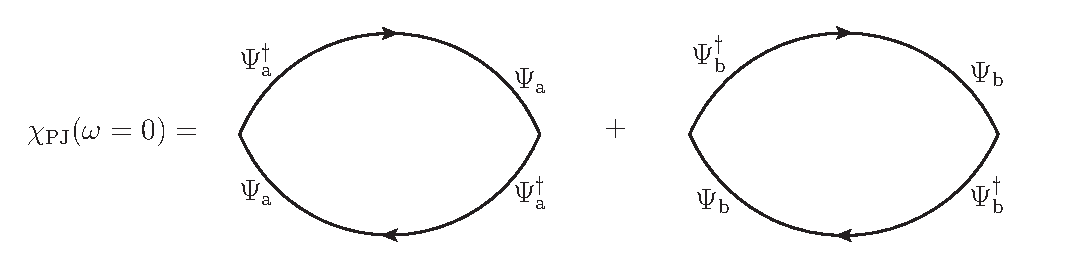
\includegraphics[width=0.8\textwidth]{static_susceptibility.eps}
	\caption{caption}
	\label{fig: static susceptibility}
\end{figure}
%
%
\begin{align}
	\chi_{\mt{PJ}}(\omega = 0) = 
		-\frac{1}{\hbar} 
		\int\limits_{0}^{\beta} \dd{\tau} 
		\int_{\vb{k}}
		\bigg[
			&\frac{k_{j}^{2}}{m_{1}}
			\expval{
				\mathcal{T}_{\tau}
				\Psi_{\mt{a}}^{\dag}(\vb{k},\tau)
				\Psi_{\mt{a}}(\vb{k},\tau)
				\Psi_{\mt{a}}^{\dag}(\vb{k},0)
				\Psi_{\mt{a}}(\vb{k},0)
			}_{0}
			\notag \\ +
			&\frac{k_{j}^{2}}{m_{2}}
			\expval{
				\mathcal{T}_{\tau}
				\Psi_{\mt{b}}^{\dag}(\vb{k},\tau)
				\Psi_{\mt{b}}(\vb{k},\tau)
				\Psi_{\mt{b}}^{\dag}(\vb{k},0)
				\Psi_{\mt{b}}(\vb{k},0)
			}_{0}
		\bigg]
\end{align}
%
\todo{Vielleicht noch etwas zu der delta-Distribution und so schreiben, damit klar is warum die Operatoren alle beim gleichen Impuls sind.}
The two expectation value of four fermionic operators can't be solved directly.
Wick's theorem offers the oppertunity to write these expectation values into a product of expectation values contained only two operators, which are nothing else free propagators.
Two contraction are possible for each expectation value in the investigated case above, where one of them vanishes, because the time argument of the contracted operator is the same.
%
\begin{align}
	\chi_{\mt{PJ}}(\omega = 0) &= 
		\frac{1}{\hbar} 
		\int\limits_{0}^{\beta} \dd{\tau} 
		\int_{\vb{k}} 
		k_{j}^{2}
		\bigg[
			\frac{1}{m_{1}}
			\mathcal{G}_{\mt{a}}^{(0)}(\vb{k},-\tau)
			\mathcal{G}_{\mt{a}}^{(0)}(\vb{k},\tau)
			+
			\frac{1}{m_{2}}
			\mathcal{G}_{\mt{b}}^{(0)}(\vb{k},-\tau)
			\mathcal{G}_{\mt{b}}^{(0)}(\vb{k},\tau)
		\bigg]
\end{align}
%
where the free fermionic propagator $\mathcal{G}_{\alpha}^{(0)}(\vb{k},\tau) = -\expval*{\mathcal{T}_{\tau} \Psi_{\alpha}(\vb{k},\tau) \Psi_{\alpha}^{\dag}(\vb{k},0)}$ with $\alpha \in \{\mt{a},\mt{b}\}$ is introduced.
The Green functions of electrons are transformed into the Matsubara frequency space, thus the only time dependence is at the exponential functions.
The $\tau$-integral yields a $\delta$-distrubution $\delta(\omega_{m} - \omega_{n})$ and then one sum over the Matsubara frequencies can be performed.
%
\begin{align}
	\chi_{\mt{PJ}}(\omega = 0) &= 
		\frac{1}{\hbar} 
		\int_{\vb{k}} 
		k_{j}^{2}
		\bigg[
			\frac{1}{m_{1}}
			S_{\mt{a}}(\omega_{n})
			+
			\frac{1}{m_{2}}
			S_{\mt{b}}(\omega_{n})
		\bigg],
\end{align}
%
where the Matsubara sum $S_{\alpha}(\omega_{n}) = \beta^{-1} \sum_{\omega_{n}} \mathcal{G}_{\alpha}^{(0)}(\vb{k},\omega_{n}) \mathcal{G}_{\alpha}^{(0)}(\vb{k},\omega_{n})$ is introduced.
The Matsubara theory exhibits that these kinds of sums can be evaluated by rewriting the sum as a contour integral in the complex plane, integrating over the Green function multiplied with the Fermi or Bose distribution caused by the nature of the Green function.
This transformation yields
%
\begin{align}
	S = \frac{1}{\beta} \sum\limits_{\omega_{n}} \mathcal{G}(\omega_{n}) = -\frac{1}{2\pi i} \oint_{\Gamma} \dd{z} n_{\mt{F}}(z) \mathcal{G}(z)
\end{align}
%
%
\begin{figure}
	\centering
	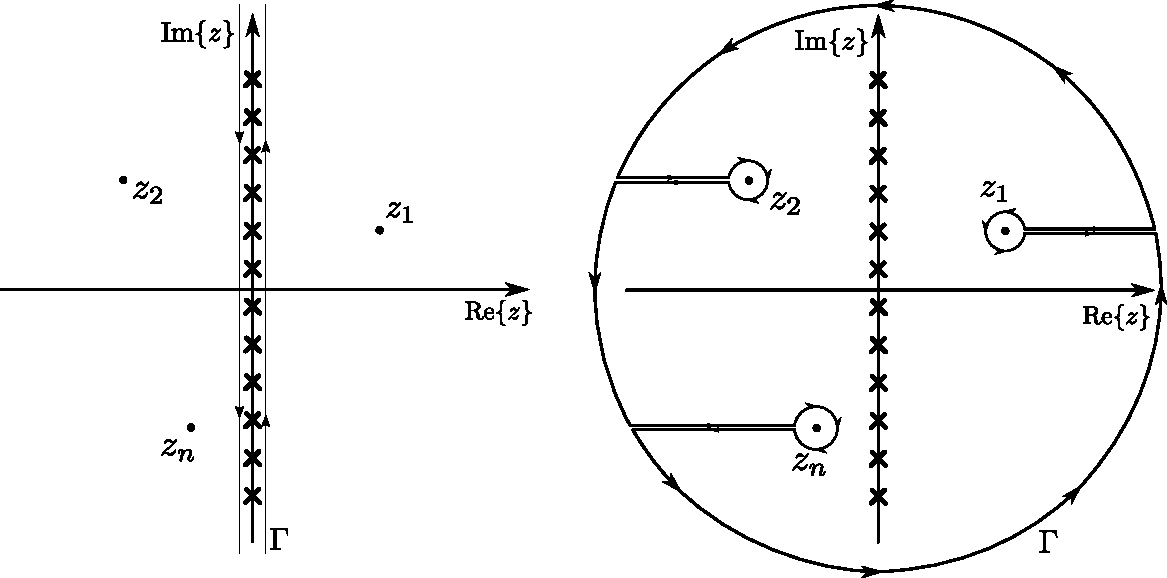
\includegraphics[width=0.8\textwidth]{contour_simple_poles.pdf}
	\caption{caption}
	\label{fig: contour simple poles}
\end{figure}
%
in the case of a fermionic Green function.
Thereby the contour is arbitrary.
The only important fact is that all singularities of the Green function has to be excluded of the contour.
Only the singularities of the distribution function are included in the contour.
The contour $\Gamma$ is expanded to infinity, where always the singularities of the Green function has to be excluded.
This procedure is depicted in figure \ref{fig: contour simple poles}.
The paths from infinity to the poles and back yield the same contribution beside the sign, why both cancel each outher.
The contour is therefore deformed to circles around the poles running clockwise and an infinite circle running counterclockwise.
The latter is zero, because the Green function is proportional to $\flatfrac{1}{z}$.
The electronic Green function is given by
%
\begin{align}
	\mathcal{G}_{\alpha}(\vb{k},\omega_{n}) = \frac{1}{i\omega_{n} - \epsilon_{\alpha}(\vb{k})},
\end{align}
%
where $\epsilon_{\alpha}(\vb{k})$  is the electron's dispersion relation with respect to the corresponding Fermi suface denoted with a and b (see equation \dots \todo{Link zu den Dispersionsrelationen}), has only simple poles in the complex plane, which means the function is continously in the whole complex plane.
Therefore the well known residuum theorem can be used to evaluate the contour integral.
%
\begin{align}
	\chi_{\mt{PJ}}(\omega = 0) &= 
		-\frac{1}{\hbar} 
		\int_{\vb{k}} 
		k_{j}^{2}
		\bigg[
			\frac{1}{m_{1}}
			\dv{n_{\mt{F}}(\epsilon_{\mt{a}}(\vb{k}))}{\epsilon_{\mt{a}}(\vb{k})}
			+
			\frac{1}{m_{2}}
			\dv{n_{\mt{F}}(\epsilon_{\mt{b}}(\vb{k}))}{\epsilon_{\mt{b}}(\vb{k})}
		\bigg]
\end{align}
%
The derivatives of the distribution function with respect to the dispersion relation appears because the singularity of the Green function at $z_{0} = \epsilon_{\alpha}(\vb{k})$ is a singularity of second order.
These two integrals are exactly solvable.
Therefore the inetegrals are transformed into polar coordinates.
The transformation rule is given by $(k_{x}, k_{y}) = (q\sqrt{2m_{1,2}}\cos(\phi), q\sqrt{2m_{2,1}}\sin(\phi))$, where two forms are used, because of the different dispersion relation.
The $k_{j}^{2}$-term originates the only angular dependence, which yields $\cos[2](\phi)$ or $\sin[2](\phi)$ for the $x$- or $y$-direction, respectivily.
Because the limits of the integral are $0$ and $2\pi$ the integral yields the same result in both cases.
The upper limit of the $q$-integral can be set to infity, because the integrand is decreased very fast to zero for large values of $q$.
%
\begin{align}
	\chi_{\mt{PJ}}(\omega = 0) = 
		\frac{8 \beta \pi}{(2\pi)^{2} \hbar} \sqrt{m_{1} m_{2}}
		\int\limits_{0}^{\infty} \dd{q}
		q^{3} \frac{e^{\beta(q^{2} - \mu)}}{(e^{\beta(q^{2} - \mu)} + 1)^{2}}
\end{align}
%
The obtained integral can be solved by substituting $x = \beta(q^{2} - \mu)$.
Thereby the first of the two integrals is evaluated with integration by parts
In the second integral the integrand is equal to the derivative of the Fermi distributation.
All in one the static susceptibility of P and J is given by
%
\begin{align}
	\chi_{\mt{PJ}}(\omega = 0) = \frac{\sqrt{m_{1} m_{2}}}{\pi \beta \hbar}\ln(e^{\beta \mu} + 1)
\end{align}
%
in first order pertubation theory. \todo{Heisst es nullte oder erste Ordnung St\"orungstheorie?}
In the case of $\mu \gg k_{\mt{B}} T$ the argument of the exponential function is very large.
Therefore the one is neglectable in the argument of the logarithm and $\ln(e^{\beta\mu} + 1) \approx \beta\mu$.
In the limit of small temperatures the susceptibility is given by
%
\begin{align}
	\chi_{\mt{PJ}}(\omega = 0) \to \frac{\mu \sqrt{m_{1} m_{2}}}{\pi \hbar} \qquad (T \to 0)
\end{align}
%
The static susceptibility between P and J is temperature independent in the limit of $\mu \gg k_{\mt{B}} T$, like exactly we have expected.











































